% !TEX root = paper.tex
\begin{comment}
\section{Analysing preferred paths in $\TZE$}
For each segment $xy$ in \SBFS$(t)$ (with $y$ closer to $t$ than $x$),
we store the shortest path from $x$ to $t$ avoiding vertex $y$ (and $t_x$)
in $\TZE(xy)$. Note that the size of $|\ \{ \TZE(xy) |\ xy \ \text{is a segment in \SBFS($t$)} \}|$
is $O(\sigma) = O(\sqrt{n \sigma})$.

However, this data-structure in itself will not be able to answer query
$\QQ(s,t,u)$ where $u$ is an intersection point. We will expand  say
more on this issue in the next section.
\end{comment}
%By definition, \SBFS$(t)$ has $O(\sigma)$ intersection vertices. So, we can
%store the preferred replacement path that avoid these intersection vertices
%in a balaced binary search tree $\BST_1(t)$. In Section \ref{sec:data},
%we will see how to use this data-structure.
%Given a query $\textsc{Q}(s,t,u)$,
%we first check if $u$ is an intersection vertex in \SBFS$(t)$. If yes, in $\tilde O(1)$
%time, we return the preferred replacement path corresponding to the intersection
%vertex $u$. The space taken by $\BST_1(t)$ is $O(\sigma) = O(\sqrt{n \sigma})$.

\iflong
\else
\vspace{-2mm}
\fi
\section{Analysing preferred replacement paths in $\TON$}
\label{sec:multi1}
We first show the following:
\begin{lemma}
\label{lem:allsame}
For each segment $xy \in$ \SBFS$(t)$, $|\TON(xy)| = 1$
\end{lemma}
\iflong
\begin{proof}
  %Let $t_x$ be the vertex in $\TT$ closest to
  %$t$ on $xt$ path. Remember that we are looking at the case
  %when the replacement path avoids $t_x$, that is, the replacement
  %path merges back on $t_xt$ path.
  Assume that there are two preferred paths
   $P$ and $P'$ whose detour start in $xy$ and their avoided edge $e$ and
  $e'$(respectively) lie in $yt_x$. Since we are analyzing
  paths in the {\em far case},  detours of $P$ and $P'$ meet $xt$ path in $t_xt$ subpath.
  Since both $e$ and $e'$ lie on $yt_x$ path,
  this implies that both $P$ and $P'$ avoid $e$ and $e'$.
  Thus, we will choose the smaller of the two paths as the preferred path avoiding both
  $e$ and $e'$. Else if $|P| = |P'|$, then we will choose that path which leaves the $xt$
  path as early as possible. Thus, there is only one preferred path avoiding both
  $e$ and $e'$, a contradiction.
  \end{proof}
\fi

%Viewed from the vantage point of intersection vertex $x$, the above lemma implies that
%there is no difference between preferred path (in $\TON$) whose detour start in $xy$.
%This is due to the fact that suffix of these path are same once they hit $x$.
%So, we only need to store this common suffix (starting from $x$) for paths in $\TON$ per segment.
%We will exploit this feature of $\TON$ when we build our data-structure in Section \ref{sec:data}
%Let $\TON(xy)$ denote the preferre replacement path from $x$ to $t$ which avoids all
%edges in $yt_x$. Note that the size of $|\{ \TON(xy) |\ xy \ \text{is a segment in \SBFS($t$)} \}|$
\noindent The above lemma implies that $|\TON| = \cup_{xy \in \text{\SBFS($t$)}} |\TON(xy)| =
O(\sigma) = O(\sqrt{n \sigma})$.
%We will see that this data-structure in itself will not be able to answer query
%$\QQ(s,t,e)$. We will defer this discussion till the next section.




%\section{SIMULATION RESULTS}
\label{sec:examples}
This section presents simulation results of the proposed method implemented on the unicycle model example.
Each semidefinite program was prepared using a custom software toolbox and the modeling tool YALMIP \cite{lofberg2004yalmip}.
The programs are run with commercial solver MOSEK on a machine with $1$ TB availabe memory. 

\subsection{FRS Computation}
We computed the FRS for a 3$^\text{rd}$ order Taylor-expanded Dubins car as the low-fidelity model $f_s$.
Trajectories produced by this model were tracked by the unicycle model from Equation \eqref{eq:big_dyn} as the high-fidelity model $f$.
The vehicle's representation as an initial distribution $X_0 \subset X_s$, was a rectangle of length $0.2$ [m] in $x$ and width $0.1$ [m] in $y$, at $0^\circ$ initial heading, and centered at $x=-0.75$ and $y=0$.
This is the same vehicle representation shown in all previous figures.

% The error function $g$, illustrated in Figure \ref{fig:error_dynamics}, was given by:
% \begin{equation}
% \label{eq:g_definition}
% g(t,x_s) = \begin{bmatrix}
% v_\text{err}\cdot(1 - \frac{1}{2}\theta^2)  \\
% v_\text{err}\cdot(\theta - \frac{1}{6}\theta^3) \\
% \dot{\theta}_\text{err}
% \end{bmatrix}
% \end{equation}
% where $v_\text{err} = (t-1)^2$ and $\dot{\theta}_\text{err} = (t-1)^4$.
We chose $\tau_\text{stop} = \tau_\text{plan} = 0.5$ [s], so $T = 1$ [s].
The stopping time can be seen in Figure \ref{fig:error_dynamics}. 
The FRS computation took 79 hours and used a maximum of 150 GB of memory 
%on a server with 1 TB of available memory and 18 processors each running at 1.2 GHz.

\subsection{Set Intersection and Trajectory Planning}

We used the precomputed FRS for safe trajectory planning in $1000$ simulated trials in MATLAB on the aforementioned machine.
For each trial, the vehicle began at the same initial location and heading, surrounded by $1-10$ randomized obstacles and a randomly-located goal to reach.
%If the planning time took more than $\tau_\text{plan}$, the simulation paused until the computation was complete. 
%In practice, if $\tau_\text{plan}$ was exceeded the vehicle could begin braking to ensure safety.
The vehicle's initial speed, and the desired speed to maintain for the duration of the trial, were randomly chosen between $0.25$ and $0.75$ [m/s].
% The trials ran in 12.7 hours.
% Prior to running these trials, several example trials were run on a laptop with a 2.3 GHz processor and 16 GB of RAM.
% The trials run on the server were individually no faster than running on the laptop, because the set intersection optimization is a single-core process that uses very little memory. 
% Therefore, the server did not provide any significant decrease in the implemented planning time.


Obstacles were represented as line segments between $0.1$ and $0.2$[m] in length, with random location and orientation.
The obstacles were always placed between the vehicle and the goal.
We checked for crashes conservatively for each trial, by inspecting if any obstacle was within a circle circumscribing the rectangular vehicle at any point of the vehicle's trajectory. 
Using this method, \emph{no crashes were detected in any trial}.
Out of all the trials, $82\%$ reached the goal, and $15\%$ performed an emergency braking maneuver (by setting $v_\text{des} = 0$). 
The remaining 3\% hit a simulation iteration limit.
Examples of the vehicle's path from a randomly-generated trial and from two constructed emergency braking cases are shown in Figure \ref{fig:example_trial}.


\begin{figure}
\centering
\includegraphics[width=1\columnwidth]{running_examples.pdf}
\caption{The top subplot shows an example result out of the $1000$ trials.
This trial used eight randomly-generated obstacles.
The vehicle begins on the left at $x = -0.75$ and reaches a randomly-generated goal near $(2.5, 0.5)$, plotted as a blue circle.
Every $\tau_\text{plan} = 0.5$[s], the vehicle replans its trajectory, shown by an asterisk plotted on the global trajectory in blue.
The bounding box of the vehicle at each planning step is shown as a grey rectangle. In the bottom-left subplot, an obstacle was constructed between the vehicle and the goal, forcing an emergency braking maneuver. In the bottom-right subplot, an obstacle was constructed with a hole that would allow the vehicle to pass, but the set intersection result is overly conservative, resulting in a braking maneuver.}
\label{fig:example_trial}
\end{figure}

Currently, our implementation cannot consistently achieve $\tau_\text{plan} = 0.5$ [s].
Consequently, instead of replanning and driving simultaneously, we pause time every 0.5 [s] of the simulation to guarantee that the vehicle can finish replanning.
In a physical implementation, if $\tau_\text{plan}$ is exceeded, then the vehicle must emergency brake; recall that a safe braking trajectory is always available.
As shown in Figure \ref{fig:planning_time_vs_Nobs}, $\tau_\text{plan}$ scales linearly with the number of obstacles.
%Methods for reducing the set intersection to meet $\tau_\text{plan}$ will be presented in future work.

\begin{figure}
\centering
\includegraphics[scale=0.45,trim={1cm 6cm 1cm 7cm},clip]{planning_time_vs_Nobs.pdf}
\caption{The mean set intersection time (top) and trajectory optimization time (bottom) versus the number of obstacles. Over the $1000$ trials, each number of obstacles from $1$ to $10$ was used for $100$ trials. Notice that set intersection takes up to $3$[s], and scales with the number of obstacles. On the other hand, the trajectory optimization takes around $80$ [ms] and has low correlation with number of obstacles.}
\label{fig:planning_time_vs_Nobs}
\end{figure}

% \begin{figure}
% \centering
% \includegraphics[scale=0.5,trim={1cm 8cm 1cm 8cm},clip]{example_trial_bluecar.pdf}
% \caption{An example result out of the 1000 trials.
% This trial used eight randomly-generated obstacles.
% The vehicle begins on the left at $x = -0.75$ and reaches a randomly-generated goal near $(2.5, 0.5)$, plotted as a blue circle.
% Every $\tau_\text{plan} = 0.5$ [s], the vehicle replans its trajectory, shown by an asterisk plotted on the global trajectory in blue.
% The bounding box of the vehicle at each planning step is shown as a grey rectangle.}
% \label{fig:example_trial}
% \end{figure}

% \begin{figure}
% \centering
% \includegraphics[scale=0.4,trim={1cm 7cm 1cm 7cm},clip]{example_emergency_brake.pdf}
% \caption{An example of a forced emergency braking situation. The vehicle cannot find a path to the desired location (plotted as a blue circle), so it brakes.}
% \label{fig:example_emergency_brake}
% \end{figure}

% \begin{figure}
% \centering
% \includegraphics[scale=0.4,trim={1cm 7cm 1cm 7cm},clip]{example_overly_conservative.pdf}
% \caption{An example of an unnecessary emergency braking situation. The vehicle cannot find a path to the desired location despite an obviously-safe path existing, because the FRS is overly conservative.}
% \label{fig:example_overly_conservative}
% \end{figure}

\iflong
\else
\vspace{-2mm}
\fi
\section{Analysing preferred replacement paths in $\TTW$}
\label{sec:multi2}

%Let $xy$ be a segment in \SBFS($t$).
%Consider all the replacement that start in $xy$ and are in $\TTW$.
%Since we know that the detours of these path start in $xy$, (similar to $\TON$) we can view
%these replacement paths as if they are starting from $a$.

We first show that one special kind of path will never lie in $\TTW$.
This characterization will help in analyzing bad paths in $\TTW$.


\begin{lemma}
\label{lem:feature}
Let $P$ be a preferred path from $x$ to $t$ avoiding $e$ on $xt$ path.
If $P$ merges with any segment $x'y'$ and then diverges from $x't$ path, then $P \notin \TTW$.
\end{lemma}
\iflong
  \begin{figure}[hpt!]
\centering
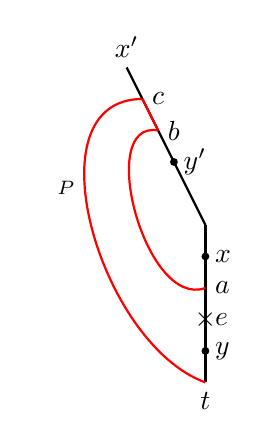
\begin{tikzpicture}[scale=2]
\begin{scope}
\coordinate (s) at (-0.5,2);
\coordinate (s1) at (0.5,2);
\coordinate (w) at (0,1);
\coordinate (t) at (0,0);
\coordinate (x) at (0,0.8);
\coordinate (y) at (0,0.2);
\coordinate (y1) at (-0.2,1.4);
\coordinate (i1) at (-0.4,1.8);
\coordinate (i2) at (-0.3,1.6);
\coordinate (a) at (0,0.6);
\coordinate (v) at (0,0.4);



\draw[thick](s)--(w);
%\draw[thick](s1)--(w);
\draw[thick](w)--(t);
\node[above] at (s){$x'$};
%\node[above] at (s1){$s$};
\node[below] at (t){$t$};

\node[right] at (a){$a$};

%\node[right] at (w){$w$};
\node[right] at (i1){$c$};
\node[right] at (i2){$b$};


\draw[red,thick] (a) to[out=200,in=170]
(i2);
\draw[red,thick](i1)--(i2);
\draw[red,thick] (i1) to[out=180,in=160]node[pos=0.4,left,black]{\scriptsize{$P$}}  (t);
\node at (v){$\times$};
\node[right] at (v){$e$};
\draw (y) node[fill,circle,scale=0.3]{};
\node[right] at (y){$y$};
\draw (x) node[fill,circle,scale=0.3]{};
\node[right] at (x){$x$};
\draw (y1) node[fill,circle,scale=0.3]{};
\node[right] at (y1){$y'$};
\end{scope}
\end{tikzpicture}
\caption{The path $P$ merges with another segment $x'y'$  and then diverges.}
\label{fig:feature}

\end{figure}

  \begin{proof}
  Once $P$ merges with $x'y'$ segment, it will diverge from it only if
  $x't$ contains $e$. This implies that $xt$ and $x't$ intersect or $xt$
  is a subpath of $x't$.
  %If $\DET(P)$ starts on $sw$ path
  %(before or on the intersection vertex $w$), then $P \in \TON$.
  %We will argue now that $\DET(P)$
  %cannot start after the intersection vertex.

  \noindent Assume for contradiction that $P \in \TTW$, that is, $\DET(P)$
  start strictly inside segment $xy$. Consider the Figure \ref{fig:feature} in which
  the detour of the preferred replacement path $P$
  starts after $x$ (at $a$). It then intersect  $x'y'$ at $b$
  and then diverges from $x't$ path at $c$.
  We claim that there exists another path to reach $b$ that is shorter  than
  $xa \conc ab$. This path is $xb$, where path $xb$ is a subpath of $x't$.
  It is also a shorter path (in $G_p$) as it uses
   edges in original $x't$ path.

  This path (1) diverges at $x$ and (2) is shorter (in $G_p$) as it uses edges from $x't$ path.
  Thus, there is a shorter replacement path than $P$ that avoids $e$. This path is not in
  $\TTW$ as its detour starts at $x$  .
  This leads to a contradiction as we had assumed that $P$ is the preferred replacement path avoiding $e$.
  Thus our assumption,
  namely that $P \in \TTW$ must be false.
  \end{proof}
\fi

\noindent We will now analyze  paths in $\TTW$. Consider two replacement
paths $P, P'$ avoiding edges $e,e'$ (respectively) on $xy,x'y'$ segment respectively.
%($ x,x'$  are intersection vertices in \SBFS($t$)) .
Let  $a,a'$ be the starting vertex of $\DET(P), \DET(P')$ respectively.
We say that $P \prec P'$ if $|at| < |a't|$.
If $|at| = |a't|$, then the tie is broken arbitrarily.


\noindent  Given a path $P \in \TTW$, let $(< P)$ be the set of all replacement
paths in $\TTW$ that are $\prec P$ in the ordering. Similarly, $(> P)$ is
the set of all replacement paths $P' \in \TTW$ for which $P \prec P'$.
Define $\UNQ(P)$ according to this ordering (see definition \ref{def:unique}).
Assume that we are processing a replacement path $P$ according to this ordering.
If $|\UNQ(P)| \ge \sqrt{n/\sigma}$, then we can associate $O(\sqrt{n/\sigma})$
{\em unique} vertices to $P$. Otherwise $|\UNQ(P)| < \sqrt{n/\sigma}$ and we have the following two cases:

\iflong
\else
\vspace{-2mm}
\fi



\subsection{ $\DET (P)$ does not intersect with any other detour in $(> P)$ }
\label{subsec:nointersect}
\noindent This case is similar to the first case in Section \ref{subsec:singlecaseone}.
\iflong
  Assume that $P$ avoids an edge $e$ on segment $xy$. Let $\DET(P)$
  start at $a \in xy$ and end at $b$ -- the vertex
  where it touches $t_xt$ path. Let $ab$ denote the
path from $a$ to $b$ on $P$. By our assumption $\UNQ(P)
  = ab$ and $|ab| < \sqrt{n/\sigma}$. Consider the following set
  of replacement paths  $(< P)_x := \{P' \in (< P)\ |\ P'~ \text{avoids an edge on $xy$ segment}\}$.
  By Lemma \ref{lem:avoids},
  all  replacement paths in $(< P)_x$ pass through $e$ (as
  detour of these replacement paths start below $e$) and by
  Lemma \ref{lem:avoidreverse}, these replacement paths avoid
  edges that are closer to $y$ than $e$. We can view these
  replacement paths as if they are starting from vertex $a$.
   $|P \setminus xa|
  = |ab| + |bt| \le \sqrt {n/\sigma} + |at|$. Using lemma \ref{lem:length}, total
  number of paths in   $(\le P)_x$ is  $\le \sqrt{ n/\sigma}$.  Thus, once we
  get a replacement path $P \in \TTW(xy)$ with $|\UNQ(P)| < \sqrt{n /\sigma}$, then there
  are at most $\sqrt{n/\sigma}$ replacement paths in $\TTW(xy)$ remaining to be processed.
  Thus, total number of paths in $\TTW$ with  $|\UNQ(P)|< \sqrt{n/\sigma}$ is
  $\sum_{xy \in \text{\SBFS($t$)}} \sqrt{n/ \sigma} = O(\sqrt{n \sigma})$
  (as there are $O(\sigma)$ segments in \SBFS($t$))
\else
   We can show that once we
   get a replacement path $P \in \TTW(xy)$ with $|\UNQ(P)| < \sqrt{n /\sigma}$, then there
   are at most $O(\sqrt{n/\sigma})$ replacement paths in $\TTW(xy)$ remaining to be processed. This will bound
   the total number of such paths to $O(\sqrt{n\sigma})$. Please see
   the full version for details.
\fi

\iflong
\else
\vspace{-2mm}
\fi
\subsection{ $\DET(P)$ intersects with  detour of a  path in $(> P)$}
\label{subsec:pintersects}

We first give a formal definition of a bad path that was defined informally in Section \ref{sec:problem}.
\begin{definition} (Bad Path)
A path $P \in \TTW$ is called a bad path if there exists another path $P' \in (>P)$
such that (1) $\DET(P)$ intersects with $\DET(P')$ and (2) $\DET(P')$ passes through the edge
avoided by $P$ after their intersection. We also say that $P$ is a bad replacement
path due to $P'$ if $P'$ satisfies the above two conditions.
\end{definition}

A path that is not bad is called a good path. In Section \ref{sec:problem}, we saw that
bad paths break the easy analysis of the single source case.
So, we have two cases depending on whether the path is good or bad. Let us look at the easier case first.\iflong\\\else\vspace{1mm}\fi


% Note that our analysis in Section \ref{sec:avoids} was easy as $P'$ cannot pass through $e$.
%However, as we have seen in Section \ref{sec:problem}, $P'$ can pass through $e$.
%Let us first look at the scenario when $P'$ does not pass through $e$ after intersection with $P$.
\iflong
\else
\section{SIMULATION RESULTS}
\label{sec:examples}
This section presents simulation results of the proposed method implemented on the unicycle model example.
Each semidefinite program was prepared using a custom software toolbox and the modeling tool YALMIP \cite{lofberg2004yalmip}.
The programs are run with commercial solver MOSEK on a machine with $1$ TB availabe memory. 

\subsection{FRS Computation}
We computed the FRS for a 3$^\text{rd}$ order Taylor-expanded Dubins car as the low-fidelity model $f_s$.
Trajectories produced by this model were tracked by the unicycle model from Equation \eqref{eq:big_dyn} as the high-fidelity model $f$.
The vehicle's representation as an initial distribution $X_0 \subset X_s$, was a rectangle of length $0.2$ [m] in $x$ and width $0.1$ [m] in $y$, at $0^\circ$ initial heading, and centered at $x=-0.75$ and $y=0$.
This is the same vehicle representation shown in all previous figures.

% The error function $g$, illustrated in Figure \ref{fig:error_dynamics}, was given by:
% \begin{equation}
% \label{eq:g_definition}
% g(t,x_s) = \begin{bmatrix}
% v_\text{err}\cdot(1 - \frac{1}{2}\theta^2)  \\
% v_\text{err}\cdot(\theta - \frac{1}{6}\theta^3) \\
% \dot{\theta}_\text{err}
% \end{bmatrix}
% \end{equation}
% where $v_\text{err} = (t-1)^2$ and $\dot{\theta}_\text{err} = (t-1)^4$.
We chose $\tau_\text{stop} = \tau_\text{plan} = 0.5$ [s], so $T = 1$ [s].
The stopping time can be seen in Figure \ref{fig:error_dynamics}. 
The FRS computation took 79 hours and used a maximum of 150 GB of memory 
%on a server with 1 TB of available memory and 18 processors each running at 1.2 GHz.

\subsection{Set Intersection and Trajectory Planning}

We used the precomputed FRS for safe trajectory planning in $1000$ simulated trials in MATLAB on the aforementioned machine.
For each trial, the vehicle began at the same initial location and heading, surrounded by $1-10$ randomized obstacles and a randomly-located goal to reach.
%If the planning time took more than $\tau_\text{plan}$, the simulation paused until the computation was complete. 
%In practice, if $\tau_\text{plan}$ was exceeded the vehicle could begin braking to ensure safety.
The vehicle's initial speed, and the desired speed to maintain for the duration of the trial, were randomly chosen between $0.25$ and $0.75$ [m/s].
% The trials ran in 12.7 hours.
% Prior to running these trials, several example trials were run on a laptop with a 2.3 GHz processor and 16 GB of RAM.
% The trials run on the server were individually no faster than running on the laptop, because the set intersection optimization is a single-core process that uses very little memory. 
% Therefore, the server did not provide any significant decrease in the implemented planning time.


Obstacles were represented as line segments between $0.1$ and $0.2$[m] in length, with random location and orientation.
The obstacles were always placed between the vehicle and the goal.
We checked for crashes conservatively for each trial, by inspecting if any obstacle was within a circle circumscribing the rectangular vehicle at any point of the vehicle's trajectory. 
Using this method, \emph{no crashes were detected in any trial}.
Out of all the trials, $82\%$ reached the goal, and $15\%$ performed an emergency braking maneuver (by setting $v_\text{des} = 0$). 
The remaining 3\% hit a simulation iteration limit.
Examples of the vehicle's path from a randomly-generated trial and from two constructed emergency braking cases are shown in Figure \ref{fig:example_trial}.


\begin{figure}
\centering
\includegraphics[width=1\columnwidth]{running_examples.pdf}
\caption{The top subplot shows an example result out of the $1000$ trials.
This trial used eight randomly-generated obstacles.
The vehicle begins on the left at $x = -0.75$ and reaches a randomly-generated goal near $(2.5, 0.5)$, plotted as a blue circle.
Every $\tau_\text{plan} = 0.5$[s], the vehicle replans its trajectory, shown by an asterisk plotted on the global trajectory in blue.
The bounding box of the vehicle at each planning step is shown as a grey rectangle. In the bottom-left subplot, an obstacle was constructed between the vehicle and the goal, forcing an emergency braking maneuver. In the bottom-right subplot, an obstacle was constructed with a hole that would allow the vehicle to pass, but the set intersection result is overly conservative, resulting in a braking maneuver.}
\label{fig:example_trial}
\end{figure}

Currently, our implementation cannot consistently achieve $\tau_\text{plan} = 0.5$ [s].
Consequently, instead of replanning and driving simultaneously, we pause time every 0.5 [s] of the simulation to guarantee that the vehicle can finish replanning.
In a physical implementation, if $\tau_\text{plan}$ is exceeded, then the vehicle must emergency brake; recall that a safe braking trajectory is always available.
As shown in Figure \ref{fig:planning_time_vs_Nobs}, $\tau_\text{plan}$ scales linearly with the number of obstacles.
%Methods for reducing the set intersection to meet $\tau_\text{plan}$ will be presented in future work.

\begin{figure}
\centering
\includegraphics[scale=0.45,trim={1cm 6cm 1cm 7cm},clip]{planning_time_vs_Nobs.pdf}
\caption{The mean set intersection time (top) and trajectory optimization time (bottom) versus the number of obstacles. Over the $1000$ trials, each number of obstacles from $1$ to $10$ was used for $100$ trials. Notice that set intersection takes up to $3$[s], and scales with the number of obstacles. On the other hand, the trajectory optimization takes around $80$ [ms] and has low correlation with number of obstacles.}
\label{fig:planning_time_vs_Nobs}
\end{figure}

% \begin{figure}
% \centering
% \includegraphics[scale=0.5,trim={1cm 8cm 1cm 8cm},clip]{example_trial_bluecar.pdf}
% \caption{An example result out of the 1000 trials.
% This trial used eight randomly-generated obstacles.
% The vehicle begins on the left at $x = -0.75$ and reaches a randomly-generated goal near $(2.5, 0.5)$, plotted as a blue circle.
% Every $\tau_\text{plan} = 0.5$ [s], the vehicle replans its trajectory, shown by an asterisk plotted on the global trajectory in blue.
% The bounding box of the vehicle at each planning step is shown as a grey rectangle.}
% \label{fig:example_trial}
% \end{figure}

% \begin{figure}
% \centering
% \includegraphics[scale=0.4,trim={1cm 7cm 1cm 7cm},clip]{example_emergency_brake.pdf}
% \caption{An example of a forced emergency braking situation. The vehicle cannot find a path to the desired location (plotted as a blue circle), so it brakes.}
% \label{fig:example_emergency_brake}
% \end{figure}

% \begin{figure}
% \centering
% \includegraphics[scale=0.4,trim={1cm 7cm 1cm 7cm},clip]{example_overly_conservative.pdf}
% \caption{An example of an unnecessary emergency braking situation. The vehicle cannot find a path to the desired location despite an obviously-safe path existing, because the FRS is overly conservative.}
% \label{fig:example_overly_conservative}
% \end{figure}

\fi
\iflong\section{SIMULATION RESULTS}
\label{sec:examples}
This section presents simulation results of the proposed method implemented on the unicycle model example.
Each semidefinite program was prepared using a custom software toolbox and the modeling tool YALMIP \cite{lofberg2004yalmip}.
The programs are run with commercial solver MOSEK on a machine with $1$ TB availabe memory. 

\subsection{FRS Computation}
We computed the FRS for a 3$^\text{rd}$ order Taylor-expanded Dubins car as the low-fidelity model $f_s$.
Trajectories produced by this model were tracked by the unicycle model from Equation \eqref{eq:big_dyn} as the high-fidelity model $f$.
The vehicle's representation as an initial distribution $X_0 \subset X_s$, was a rectangle of length $0.2$ [m] in $x$ and width $0.1$ [m] in $y$, at $0^\circ$ initial heading, and centered at $x=-0.75$ and $y=0$.
This is the same vehicle representation shown in all previous figures.

% The error function $g$, illustrated in Figure \ref{fig:error_dynamics}, was given by:
% \begin{equation}
% \label{eq:g_definition}
% g(t,x_s) = \begin{bmatrix}
% v_\text{err}\cdot(1 - \frac{1}{2}\theta^2)  \\
% v_\text{err}\cdot(\theta - \frac{1}{6}\theta^3) \\
% \dot{\theta}_\text{err}
% \end{bmatrix}
% \end{equation}
% where $v_\text{err} = (t-1)^2$ and $\dot{\theta}_\text{err} = (t-1)^4$.
We chose $\tau_\text{stop} = \tau_\text{plan} = 0.5$ [s], so $T = 1$ [s].
The stopping time can be seen in Figure \ref{fig:error_dynamics}. 
The FRS computation took 79 hours and used a maximum of 150 GB of memory 
%on a server with 1 TB of available memory and 18 processors each running at 1.2 GHz.

\subsection{Set Intersection and Trajectory Planning}

We used the precomputed FRS for safe trajectory planning in $1000$ simulated trials in MATLAB on the aforementioned machine.
For each trial, the vehicle began at the same initial location and heading, surrounded by $1-10$ randomized obstacles and a randomly-located goal to reach.
%If the planning time took more than $\tau_\text{plan}$, the simulation paused until the computation was complete. 
%In practice, if $\tau_\text{plan}$ was exceeded the vehicle could begin braking to ensure safety.
The vehicle's initial speed, and the desired speed to maintain for the duration of the trial, were randomly chosen between $0.25$ and $0.75$ [m/s].
% The trials ran in 12.7 hours.
% Prior to running these trials, several example trials were run on a laptop with a 2.3 GHz processor and 16 GB of RAM.
% The trials run on the server were individually no faster than running on the laptop, because the set intersection optimization is a single-core process that uses very little memory. 
% Therefore, the server did not provide any significant decrease in the implemented planning time.


Obstacles were represented as line segments between $0.1$ and $0.2$[m] in length, with random location and orientation.
The obstacles were always placed between the vehicle and the goal.
We checked for crashes conservatively for each trial, by inspecting if any obstacle was within a circle circumscribing the rectangular vehicle at any point of the vehicle's trajectory. 
Using this method, \emph{no crashes were detected in any trial}.
Out of all the trials, $82\%$ reached the goal, and $15\%$ performed an emergency braking maneuver (by setting $v_\text{des} = 0$). 
The remaining 3\% hit a simulation iteration limit.
Examples of the vehicle's path from a randomly-generated trial and from two constructed emergency braking cases are shown in Figure \ref{fig:example_trial}.


\begin{figure}
\centering
\includegraphics[width=1\columnwidth]{running_examples.pdf}
\caption{The top subplot shows an example result out of the $1000$ trials.
This trial used eight randomly-generated obstacles.
The vehicle begins on the left at $x = -0.75$ and reaches a randomly-generated goal near $(2.5, 0.5)$, plotted as a blue circle.
Every $\tau_\text{plan} = 0.5$[s], the vehicle replans its trajectory, shown by an asterisk plotted on the global trajectory in blue.
The bounding box of the vehicle at each planning step is shown as a grey rectangle. In the bottom-left subplot, an obstacle was constructed between the vehicle and the goal, forcing an emergency braking maneuver. In the bottom-right subplot, an obstacle was constructed with a hole that would allow the vehicle to pass, but the set intersection result is overly conservative, resulting in a braking maneuver.}
\label{fig:example_trial}
\end{figure}

Currently, our implementation cannot consistently achieve $\tau_\text{plan} = 0.5$ [s].
Consequently, instead of replanning and driving simultaneously, we pause time every 0.5 [s] of the simulation to guarantee that the vehicle can finish replanning.
In a physical implementation, if $\tau_\text{plan}$ is exceeded, then the vehicle must emergency brake; recall that a safe braking trajectory is always available.
As shown in Figure \ref{fig:planning_time_vs_Nobs}, $\tau_\text{plan}$ scales linearly with the number of obstacles.
%Methods for reducing the set intersection to meet $\tau_\text{plan}$ will be presented in future work.

\begin{figure}
\centering
\includegraphics[scale=0.45,trim={1cm 6cm 1cm 7cm},clip]{planning_time_vs_Nobs.pdf}
\caption{The mean set intersection time (top) and trajectory optimization time (bottom) versus the number of obstacles. Over the $1000$ trials, each number of obstacles from $1$ to $10$ was used for $100$ trials. Notice that set intersection takes up to $3$[s], and scales with the number of obstacles. On the other hand, the trajectory optimization takes around $80$ [ms] and has low correlation with number of obstacles.}
\label{fig:planning_time_vs_Nobs}
\end{figure}

% \begin{figure}
% \centering
% \includegraphics[scale=0.5,trim={1cm 8cm 1cm 8cm},clip]{example_trial_bluecar.pdf}
% \caption{An example result out of the 1000 trials.
% This trial used eight randomly-generated obstacles.
% The vehicle begins on the left at $x = -0.75$ and reaches a randomly-generated goal near $(2.5, 0.5)$, plotted as a blue circle.
% Every $\tau_\text{plan} = 0.5$ [s], the vehicle replans its trajectory, shown by an asterisk plotted on the global trajectory in blue.
% The bounding box of the vehicle at each planning step is shown as a grey rectangle.}
% \label{fig:example_trial}
% \end{figure}

% \begin{figure}
% \centering
% \includegraphics[scale=0.4,trim={1cm 7cm 1cm 7cm},clip]{example_emergency_brake.pdf}
% \caption{An example of a forced emergency braking situation. The vehicle cannot find a path to the desired location (plotted as a blue circle), so it brakes.}
% \label{fig:example_emergency_brake}
% \end{figure}

% \begin{figure}
% \centering
% \includegraphics[scale=0.4,trim={1cm 7cm 1cm 7cm},clip]{example_overly_conservative.pdf}
% \caption{An example of an unnecessary emergency braking situation. The vehicle cannot find a path to the desired location despite an obviously-safe path existing, because the FRS is overly conservative.}
% \label{fig:example_overly_conservative}
% \end{figure}
\fi

\noindent {(1) \em $P$ is a good path.}

\noindent Assume that $P \in \TTW(xy)$ and it avoids an edge $e \in xy$.
Assume that $P$  intersects first with $P' \in (> P)$ and $P'$ avoids $e'$ on $x'y'$ segment.
Note that $x$ may be equal to $x'$.
Let $\DET(P')$ start at $a'$ and end at
$b'$. Assume that $\DET(P)$ starts at $a$ and it intersects $\DET(P')$
at $c$.
Consider the path $x'a' \conc a'c \conc ca \conc at$. Since $x'a' \conc a'c$ is a part of $P'$,
it avoids $e'$. However, it is not clear whether $ca \conc at$ avoids $e'$ too.
In Figure \ref{fig:examples}, we see two representative examples in which $ca$ and $at$
avoid $e'$.
\iflong
  We will now show that both $ca$   and $at$ cannot passes through $e'$.
  %then $P$ is {\em similar} to $P'$
  %(in which case we can discard path $P$).
  \begin{enumerate}
   \item[(a)] Assume that  $ca$ passes through $e'$ %(See Figure \ref{fig:badexample1}(a))
    \label{enum:goodcase}

  If $x=x'$, then by Lemma \ref{lem:avoids}, as $P' \in (>P)$, $\DET(P)$ (and hence $ca$)
   starts below $e'$. Thus, $ca$ cannot pass through $e'$ as $\DET(P)$ does not
  intersect $xt_x$ path and $e' \in xt_x$. So let us assume that $x \neq x'$.
  This implies that $P$ intersects $x'y'$. After intersecting $x'y'$ path
    $P$ did not follow $x'y' \conc y't$ (since $ca$ intersect $\DET(P')$ at $c$).
    %This implies that $s't$ path contains $e$ (the vertex $P$ avoids).
    %Thus, $s't$ and $st$ intersect, say at $w$ and $e$ lies after $w$ on $s't$
    %and $st$ path. Since $P \in \TTW$, $\DET(P)$ should also start after $w$.
    %Since $\DET(P)$ passes through $e'$, $e'$ cannot lie on $wt$ path
    %(as $wt$ is a subpath of $st$ and by defintion $\DET(P)$ cannot intersect $st$).
    %Thus $e' \in sw$.
    This implies that $P$ intersect with another path $x'y'$ and then
    diverges. By Lemma \ref{lem:feature}, $P \notin \TTW$.
    This leads to a contradiction as we assumed that $P \in \TTW$. Thus our
    assumption, namely $ca$ passes through
    $e'$ is false.


    %Now, we have to satisfy two conditions (1) $\DET(P)$ should start below $w$ and (2) $\DET(P)$ should pass through $w$.  We claim that $P$ cannot satisfy both the condition. This is because the best vertex for a detour to start to satisfy condition (2) is $w$, the intersection vertex of $s't$ and $st$.


    %Thus, such a $P$ cannot exists as we have reached a contradiction. So, $ca$ cannot pass through $e'$.

  \item[(b)] Assume that $at$ passes through $e'$ %(See Figure \ref{fig:badexample1}(b))
  \label{enum:one}

  If $x = x'$, then by Lemma \ref{lem:avoids}, starting vertex of $\DET(P)$, that is $a$, starts below $e'$. Thus,
  $at$ cannot pass through $e'$. So let us assume that $x \neq x'$.
  If $at$ passes through $e'$, then segment $x'y'$ is a subpath of $xt$ path.
  This is due to the fact that $a \in xy$ and $e' \in x'y'$. Since $P' \in \TTW(x'y')$,
  $\DET(P')$ starts strictly inside segment $x'y'$, at vertex $a'$. This implies that $|a't| < |at|$.
  This contradicts our assumption that $P' \in (>P)$. Thus, $at$ cannot pass through $e'$.
  %Once again $x \neq x'$
  %Since $a \in st$ and $e' \in s't$, this implies that $st$ and $s't$ intersect at $w$
  %and $e'$ lies in $wt$ path.
  %Since $P' \in \TTW$, $\DET(P')$ should also
  %start in $wt$.  Since $P' \in (>P)$, $|a't| \ge |at|$. We claim that $a't$
  %contains both $e$ and $e'$. This is due to the fact that $e \in at$, $|a't| \ge |at|$
  %and by assumption $e' \in at$.
  %Thus we have two path $P$ and $P'$ that are meet at vertex $w$ after which
  %their detour start at $a$ and $a'$ respectively and  both these detours
  %avoid $e'$ and $e$. So, the preferred path avoiding $e$ and $e'$ from $w$ is either the suffix of $P$ or $P'$ -- the one which is the shortest replacement path and leaves $wt$ path as early as possible.
  %This implies that both $P$ and $P'$ have same detour
  %and they start from the same vertex, that is $a = a'$.



  %We claim that $e$ cannot lie on $wt$ path as it then leads
  %to case \ref{}, which is known to be an easy scenario. This implies that $|at| > |a't|$. Thus, $P' \notin (>P)$. This leads to a contradiction as we started out with the assumption that $P' \in (>P)$.

  \end{enumerate}
\fi


%When viewed from the vantage point of intersection vertex
%$w$,
%there is no difference between $P$ and $P'$. Thus, we discard
%$P$.

%Thus, if $P$ is not discarded, then both $ca$ and $at$ also avoid $e'$.
\iflong\else In the full version of the paper, we show that $ca$ and $at$ cannot pass through $e'$. \fi
Thus, the path $x'a' \conc a'c \conc ca \conc at$ is indeed a valid replacement
path from $x'$ to $t$ avoiding $e'$. Since $P' = x'a' \conc a'c \conc cb' \conc b't$, length
of $P'$ must be $\le$ length of  this alternate path. Thus,\\
\begin{tabular}{llll}
& $|x'a'| +  |a'c|
+ |cb'| + |b't|$& $\le$ & $|x'a'| + |a'c| + |ca|  + |at|$  \\
$\implies$& $
|cb'| + |b't|$ & $\le$ & $|ca|  + |at|$   \\
$\implies$&$|ac| +
|cb'| + |b't|$ & $\le$ &  $2|ca|  + |at|$

\end{tabular}
%\begin{figure}
\centering
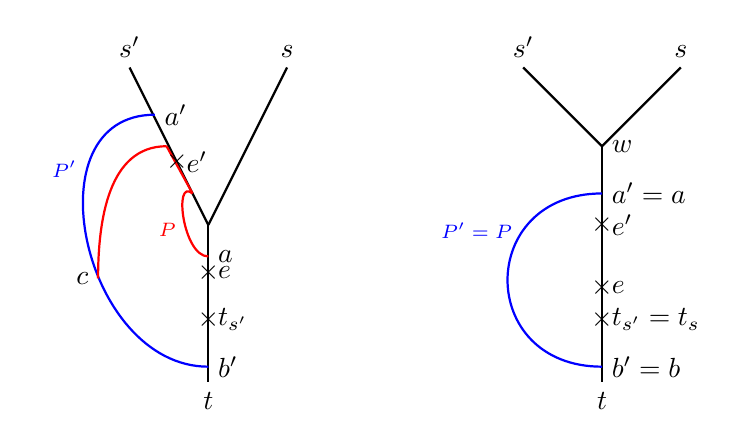
\begin{tikzpicture}[scale=2]
\begin{scope}
\coordinate (s) at (-0.5,2);
\coordinate (s1) at (0.5,2);
\coordinate (w) at (0,1);
\coordinate (t) at (0,0);
\coordinate (ts) at (0,0.4);
\coordinate (b1) at (0,0.1);

\coordinate (i1) at (-0.265,1.5);
\coordinate (i2) at (-0.1,1.2);

\coordinate (a1) at (-0.34,1.7);
\coordinate (a) at (0,0.8);
\coordinate (v) at (0,0.7);
\coordinate (v1) at (-0.2,1.4);
\coordinate (c) at (-0.7,0.66);

\draw[thick](s)--(w);
\draw[thick](s1)--(w);
\draw[thick](w)--(t);
\node[above] at (s){$s'$};
\node[above] at (s1){$s$};
\node[below] at (t){$t$};
\node[right] at (a1){$a'$};
\node[right] at (a){$a$};
\node[right] at (b1){$b'$};
\node[left] at (c){$c$};


\draw[blue,thick] (a1) to[out=180,in=180,distance=.8cm]
node[pos=0.3,left]
{\scriptsize  $P'$}  (b1);

\draw[red,thick] (a) to[out=180,in=140]
node[pos=0.4,left]
{\scriptsize  $P$}  (i2);
\draw[red,thick](i1)--(i2);
\draw[red,thick] (i1) to[out=180,in=90](c);

\node at (v1){$\times$};
\node[right] at (v1){$e'$};

\node at (v){$\times$};
\node[right] at (v){$e$};

\node at (ts){$\times$};
\node[right] at (ts){$t_{s'}$};

\end{scope}
\begin{scope}[xshift=2.5cm]
\coordinate (s) at (-0.5,2);
\coordinate (s1) at (0.5,2);
\coordinate (w) at (0,1.5);
\coordinate (t) at (0,0);
\coordinate (ts) at (0,0.4);
\coordinate (b1) at (0,0.1);

\coordinate (i1) at (-0.265,1.5);
\coordinate (i2) at (-0.1,1.2);

\coordinate (a1) at (0,1.2);
\coordinate (a) at (0.29,1.6);
\coordinate (v) at (0,0.6);
\coordinate (v1) at (0,1);
\coordinate (c) at (-0.7,0.66);

\draw[thick](s)--(w);
\draw[thick](s1)--(w);
\draw[thick](w)--(t);
\node[above] at (s){$s'$};
\node[above] at (s1){$s$};
\node[below] at (t){$t$};
\node[right] at (a1){$a'=a$};
\node[right] at (w){$w$};
\node[right] at (b1){$b'=b$};



\draw[blue,thick] (a1) to[out=180,in=180,distance=.8cm]
node[pos=0.3,left]
{\scriptsize  $P'=P$}  (b1);


\node at (v1){$\times$};
\node[right] at (v1){$e'$};

\node at (v){$\times$};
\node[right] at (v){$e$};

\node at (ts){$\times$};
\node[right] at (ts){$t_{s'} = t_s$};

\end{scope}
\end{tikzpicture}
\caption{ffs}
\label{fig:badexample1}

\end{figure}


On the left hand of the inequality, we  have a path from
$a$ to $t$ avoiding $e$ (since we know that $P$ is a good path, so $P'$ and thus $cb' \conc b't$ does not
pass through $e$). So, its length should be $\ge$
length of the preferred path $P \setminus xa$. Thus $|P
\setminus xa| \le 2|ca|  + |at| \le 2\sqrt {n/\sigma}\
+\ |at|$ (since $|\UNQ(P)| = |ac| < \sqrt{n/\sigma}$). Consider the following set of replacement paths  $(< P)_x
:= \{P' \in (< P)\ |\ P' \ \text{avoids
an edge on $xy$ segment}\}$. By Lemma \ref{lem:avoids},
all  replacement paths in $(<P)_x$ pass through $e$ (as
detour of these replacement paths start below $e$) and by
Lemma \ref{lem:avoidreverse}, these replacement paths avoid
edges that are closer to $y$ than $e$.
  Applying Lemma \ref{lem:length}, we get
that  the number of replacement paths $(<P)_x$  is $ \le 2\sqrt{n/\sigma}$. Thus, once we
get a replacement path $P \in \TTW(xy)$ with $|\UNQ(P)| < \sqrt{n /\sigma}$, then there
are at most $2\sqrt{n/\sigma}$ replacement paths in $\TTW(xy)$ remaining to be processed.
Thus, total number of paths $\in \TTW$ with  $|\UNQ(P)| < \sqrt{n/\sigma}$ is
$\sum_{xy \in \text{\SBFS($t$)}} 2\sqrt{n/\sigma} = O(\sqrt{n \sigma})$
(as there are $O(\sigma)$ segments in \SBFS($t$)).\iflong\\\else\vspace{2mm}\fi

\iflong
   \begin{figure}[hpt!]
\centering
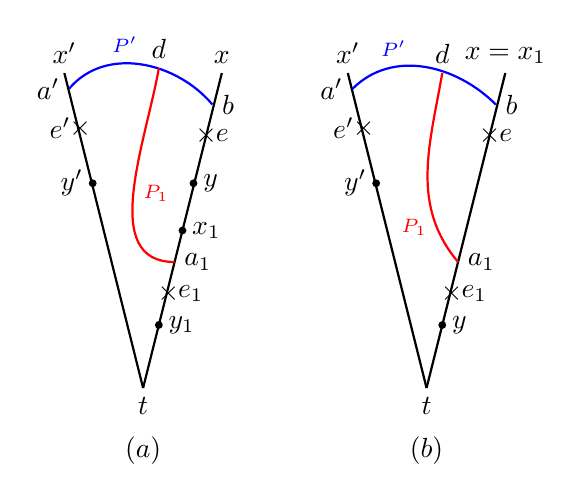
\begin{tikzpicture}[scale=2]
\begin{scope}
\coordinate (s) at (0.5,2);
\coordinate (s1) at (-0.5,2);
%\coordinate (s2) at (1.1,2);
%\coordinate (w) at (0.5,1.4);
\coordinate (t) at (0,0);
\coordinate (ts) at (0.15,0.4);
\coordinate (b) at (0.44,1.8);
\coordinate (y1) at (-0.32,1.3);
\coordinate (y) at (0.32,1.3);

\coordinate (x2) at (0.25,1);
\coordinate (y2) at (0.1,0.4);

\coordinate (a1) at (-0.47,1.9);
\coordinate (a2) at (0.2,0.8);
\coordinate (v) at (0.4,1.6);
\coordinate (v1) at (-0.4,1.65);
\coordinate (v2) at (0.16,0.6);
\coordinate (c) at (-0.7,0.66);
\coordinate (d) at (0.1,2.03);

\draw[thick](s)--(t);
\draw[thick](s1)--(t);
%\draw[thick](s2)--(w);
%\draw[thick](w)--(t);
\node[above] at (s){$x$};
\node[above] at (s1){$x'$};
%\node[above] at (s2){$s_1$};
\node[below] at (t){$t$};
\node[left] at (a1){$a'$};
\node[right] at (b){$b$};

\node[above] at (d){$d$};
%\node[right] at (w){$w$};


\draw[blue,thick] (a1) to[out=50,in=130]
node[pos=0.4,above]
{\scriptsize  $P'$}  (b);



\draw[red,thick] (a2) to[out=180,in=260]
node[pos=0.5,right]
{\scriptsize  $P_1$}  (d);

\node at (v1){$\times$};
\node[left] at (v1){$e'$};


\node[right] at (a2){$a_1$};

\node at (v){$\times$};
\node[right] at (v){$e$};

\node at (v2){$\times$};
\node[right] at (v2){$e_1$};

%\node at (ts){$\times$};
%\node[right] at (ts){$t_{s}$};

\draw (y1) node[fill,circle,scale=0.3]{};
\node[left] at (y1){$y'$};

\draw (y) node[fill,circle,scale=0.3]{};
\node[right] at (y){$y$};

\draw (x2) node[fill,circle,scale=0.3]{};
\node[right] at (x2){$x_1$};

\draw (y2) node[fill,circle,scale=0.3]{};
\node[right] at (y2){$y_1$};

\node at (0,-0.4){$(a)$};

\end{scope}
\begin{scope}[xshift=1.8cm]
\coordinate (s) at (-0.5,2);
\coordinate (s1) at (0.5,2);

\coordinate (t) at (0,0);
\coordinate (ts) at (0.1,0.4);
\coordinate (b) at (0.44,1.8);

\coordinate (a2) at (0.2,0.8);
\coordinate (d) at (0.1,2);
\coordinate (y1) at (-0.32,1.3);
\coordinate (y) at (0.1,0.4);
\coordinate (a1) at (-0.47,1.9);
\coordinate (a) at (0.1,0.8);
\coordinate (v) at (0.4,1.6);
\coordinate (v2) at (0.16,0.6);
\coordinate (v1) at (-0.4,1.65);
\coordinate (c) at (-0.7,0.66);

\draw[thick](s)--(t);
\draw[thick](s1)--(t);

\node[above] at (s){$x'$};
\node[above] at (s1){$x=x_1$};
\node[below] at (t){$t$};
\node[left] at (a1){$a'$};

\node[right] at (b){$b$};
\node[right] at (a2){$a_1$};
\node[above] at (d){$d$};

\draw[blue,thick] (a1) to[out=45,in=135]
node[pos=0.3,above]
{\scriptsize  $P'$}  (b);


\draw[red,thick] (a2) to[out=130,in=260]
node[pos=0.2,left]
{\scriptsize  $P_1$}  (d);

\node at (v1){$\times$};
\node[left] at (v1){$e'$};

\node at (v2){$\times$};
\node[right] at (v2){$e_1$};

\node at (v){$\times$};
\node[right] at (v){$e$};



\draw (y1) node[fill,circle,scale=0.3]{};
\node[left] at (y1){$y'$};

\draw (y) node[fill,circle,scale=0.3]{};
\node[right] at (y){$y$};

\node at (0,-0.4){$(b)$};
\end{scope}
\end{tikzpicture}
\caption{Two cases in which $P'$ passes through $e_1$ after intersecting with $P_1$}
\label{fig:badexample}

\end{figure}

\fi
\noindent  {(2) \em $P$ is a bad path.}
\label{enum:two}

\noindent We now arrive at our hardest scenario.
We will first show that the number of good paths in $\TTW$
is greater than
the number of bad paths in $\TTW$.
To this end, we will prove the following lemma:
\begin{lemma}
\label{lem:badpaths}
For each $P' \in \TTW$, there exists only one replacement
path $P \in \TTW$ which is bad
due to $P'$.
\end{lemma}

\iflong
  \begin{proof}

  Assume that $P$ is the preferred path
  from $x$ to $t$ avoiding $e$ on segment $xy$. Similarly, $P'$ is the preferred path from $x'$ to $t$ avoiding $e'$ on segment $x'y'$ and $P$ is bad due to $P'$. Assume for contradiction that there is one more replacement
  path $P_1$ which is bad
  due to $P'$.
  %, that is,  1)$P_1 \in \TTW \cap (<P')$ and
  %$\DET(P_1)$ intersects with $\DET(P')$ and
  %(2) $\DET(P')$ passes through the edge avoided by $P_1$
  %after their intersection.
  Let us assume that $P_1$ avoids $e_1$ on $x_1y_1$ segment.
  If $x' = x$ or $ x'= x_1$, then $\DET(P')$ cannot pass through
  $e$ or $e_1$ respectively as
  $\DET(P')$ starts before $e$ or $e_{1}$ (as $P' \in (>P)$ or $P' \in (>P_1)$) and touches $x't$ path only at $t_{x'}t$. So, let us assume
  that $x' \neq x$ and $ x' \neq x_1$.

  Since $P' \in \TTW$, by lemma \ref{lem:feature}, we know
  that it follows $xt$ path after hitting segment $xy$, say at $b$. This
  implies
  that $e_1$ also lies on the $xt$ path. Thus, $xt$ and $x_1t$
  intersect. Without loss of generality, assume that  the segment $x_1y_1$ is
  a subpath of $xt$.
  %, say at $w$.
  %Assume without loss of generality
  %that $v_1$ is closer to $t$ than $v$ on $st$ path
  %\begin{enumerate}
  %   \item   $s_1 = s$
  %Note that if $x=x_1$, then $w := x=sx_1$.
  %Without loss of generality assume that $e_1$ is closer to
  %$t$ than $e$. %or $e_1=e$.
  %We have assumed that $P'$ passes through $e$.
  %By Lemma \ref{lem:feature},
  %we know that since $P' \in \TTW$, once it  hits $st$ path
  %(say at $b)$,
  %it cannot leave it.
  %By Lemma \ref{lem:avoids}, $\DET(P_1)$ starts below $v$
  %on $st$ path.
  Let us assume that $\DET(P_1)$ starts at $a_1$ and it
  hits $P'$ at $d$.
  There are two ways for $P_1$ to reach $d$ (both avoiding
  $e_1$):
  $x_1a_1 \conc a_1d$ and $x_1b \conc bd$
  where the first path is using the detour of $P_1$ and the second path
  uses $xt$ path to reach $b$.

  Note that the second path leaves the $x_1t$ path earlier than the
  first path ($x_1$ compared to $a_1$ if $x \neq x_1$ (Figure  \ref{fig:badexample}(a)) and
  $b$ compared to $a_1$ if $x=x_1$ (Figure  \ref{fig:badexample}(a))). Even then the preferred
  path used the first alternative.
  This implies that the length of the first path
  must be {\em strictly} less than the second.  Thus,
  $|x_1a_1| + |a_1d| < |x_1b| + |bd|$. Thus,
  \begin{equation}
  |a_1d| < |db| + |bx_1| - |x_1a_1|
  \end{equation}
  $P'$ takes the following path
  $x'a' \conc a'b \conc bt$.
  But there is  an alternative path available for $P'$, it
  is $x'a' \conc a'd \conc da_1 \conc a_1t$.
  The path is a valid path avoiding $e'$ only if $a_1d$
  does not pass through $e'$. All other components of this
  path are a part of $P'$ ($a'd \in a'b$ and $a_1t \in bt$)
  .

  If $a_1d$ does not pass through $e'$, then we can show that
  the alternative path has a length less than $|P'|$, thus arriving
  at a contradiction.
  Consider the length of the alternative path:
  \begin{tabbing}
   $|x'a'| $\=$+ |a'd| + |da_1| + |a_1t|$\\
   \>$< |x'a'|+ |a'd| + |db|  + |bx_1| - |x_1a_1| + |a_1t|$
  \hspace{10mm}\ (Using  Equation (1))\\\\
  If $x \neq x'$(See Figure  \ref{fig:badexample}(a)), then
  $ |bx_1|  - |x_1a_1|
  + |a_1t| \le  |bx_1|  + |x_1a_1| + |a_1t| = |bt|$. Else if $x
  =x'$ \\
  (See Figure  \ref{fig:badexample}(b)), then $ |bx_1|  - |x_1a_1|
  + |a_1t| = -|ba_1| +\ |a_1t| \le|ba_1| +\ |a_1t| =  |bt|$ \\\\
   \>$\le |x'a'|+ |a'd| + |db| + |bt|$\\
  \>$= |x'a'|+ |a'b| + |bt|$\\
   \>$= |P'|$
  \end{tabbing}

  This leads to a contradiction as we have assumed that $P'$
  is
  the shortest path from $x'$ to $t$ avoiding $e'$.

  To end this proof, we will show that $a_1d$ cannot pass
  through $e'$.
  Assume for contradiction that $a_1d$ passes through $e'$.
  This
  implies that $\DET(P_1)$ intersects with $x'y'$ segment (as
  $e' \in x'y'$) and
  then diverges from it (as $\DET(P_1)$ intersect with $\DET(P')$
  at $d$).
  By Lemma \ref{lem:feature}, $P_1 \notin \TTW$. But this cannot
  be the
  case as we have assumed that $P_1 \in  \TTW$. Thus our assumption,
  namely $a_1d$ passes through $e'$ must be false.


  %\item $s''=s$

  %Assume without loss of generality \todo{Is this wlog fine}
  %that $e''$ lies below $e$ on $st$ path. By Lemma \ref{},
  %we know that $P'$ leaves $st$ above $e$ and merges back
  %only at $t_st$ path. Since $e' \notin t_st$, this implies
  %that $P'$ can never pass through $e'$. Thus, we arrive
  %at a contradiction.

  %\item $s_1 \neq s$

  %Since $P' \in \TTW$, by lemma \ref{lem:feature}, we know
  %that it follows $st$ path after hitting it. This implies
  %that $v_1$ also lies on the $st$ path. Thus, $st$ and $s_1t$
  %intersect, say at $w$. Assume without loss of generality
  %that $v_1$ is closer to $t$ than $v$ on $st$ path. So,
  %$P_1$ satisfies two condition: (1) It intersects with $P'$
  %and (2) The vertex avoided by $P'$ is closer to $s$ than
  %$v''$. By Lemma \ref{}, we infer than $P'' \in \TON$. Thus,
  %we again arrive at a contradiction.

  %\end{enumerate}
  \end{proof}
\fi




%We now put the above lemma to use. We use the following
%algorithm to weed out paths that satisfy case 1(b) and case
%2.

%\begin{algorithm}
%\ForEach{$P \in \TTW$ precessed according to the ordering
%$\prec$}
%{
%    $\BP \leftarrow \emptyset$; \tcp{Set of Bad Paths}

%    $\GP \leftarrow \emptyset$; \tcp{Set of Good Paths}

%    \If{$\exists$ \ \text{a path in $GP$ whose detour start
%at the same vertex as of $P$\ }}
%    {
%        continue;
%    }
%    \If{ $\exists P' \in \GP$ such that $P'$ passes through
%$e$ after intersecting $P$ }
%    {

%        $\BP \leftarrow \BP \cup  \{P\}$\;
    % }
%     \Else
%     {
%         $\GP \leftarrow \GP \cup \{P\}$\;
%     }
% }
% \end{algorithm}

% The above algorithm discards a path $P$ if there already
% exists a processed good path whose detour starts from the
% same vertex as that of $P$. This takes care of case \ref{enum:one}.
% It then removes all the replacement paths $P$ that satisfy
% the conditions in Case \ref{enum:two}. $\BP$ is the set
% of paths removed by the algorithm. For each such path, there
% exists a path $P' \in \GP$. By Lemma \ref{lem:badpaths},
% we know that each good path in $\GP$ can remove atmost one
% bad path. This implies that the number of bad paths removed
% is $\le$ number of good paths, that is $|\BP| \le |\GP|$.
% All the paths in $\GP$ do not satisfy case \ref{enum:one}
% and \ref{enum:two}. Thus, these paths satisfy  case \ref{enum:goodcase}.

The above lemma can be used to discard bad paths from $\TTW$.
For each such discarded path, there exists at least one good path.
And by the above lemma, each such good path can be used to discard
at most one bad path. Thus the number of good paths in $\TTW$
is $\ge$ number of bad paths in $\TTW$.
We have already shown that the total number of good paths in $\TTW$
is $O(\sqrt{n\sigma})$.
Thus the total number of paths in $\TTW$ is also $O(\sqrt{n\sigma})$.

% Let $wy$ be a segment in \SBFS($t$) where $y$ is closer
% to $t$ than $w$.
% Let $\TTW(w)$ denote the set of all replacement paths in
% $\TTW$ whose detour
% start in segment $wx$. $\TTW(w)$ can be implemented as a
% balanced binary
% search tree.
%  Since size of $\TTW$ is $O(\sqrt{n \sigma})$, the size of $\cup_{w \in \text{\SBFS($t)$}}\ |\TTW(w)| = O(\sqrt{n \sigma})$.
